% !Mode:: "TeX:UTF-8"
% !TEX program  = xelatex
\documentclass[a4paper]{article}
\usepackage{amsmath}
\usepackage{amssymb}
\usepackage{ctex}
\usepackage{braket}
%\usepackage[european]{circuitikz}
\usepackage{multirow}
\usepackage{float}
\usepackage{colortbl}
\usepackage{graphicx}
\usepackage{geometry}
\geometry{left=2.5cm,right=2.5cm,bottom=2.5cm,top=2.5cm}
\usepackage{physics}
\usepackage{mhchem}
\usepackage{siunitx}
\usepackage{bm}


\title{近代物理实验报告9.2:微波段电子自旋共振}
\author{xy\quad 学号\quad 匡亚明学院}
\date{2019年2月29日}
\begin{document}
\maketitle
\bibliographystyle{unsrt}
%--------main-body------------

\section{引言}
电子自旋共振(Electron Spin Resonance,简称ESR)也称电子顺磁共振(Electron Paramagnetic Resonance),是1944年由扎伏伊斯基首先观测到的,它是磁共振波谱学的一个分支。在探索物质中末偶合电子以及它们与周围原子相互作用方面,顺磁共振具有很高的灵敏度和分辨率,并且具有在测量过程中不破坏样品结构的优点。目前它在化学,物理,生物和医学等领域都获得了广泛的应用。

\section{实验目的}
\begin{enumerate}
\item 本实验的目的是在了解电子自旋共振原理的基础上,学习用微波频段检测电子自旋共振信号的方法。
\item 测定$\ce{CuSO_4 . 5H_2O}$单晶体、DPPH中电子的g因子和共振线宽。
\item 了解、掌握微波仪器和器件的应用。
\item 学习利用锁相放大器进行小信号测量的方法。
\end{enumerate}

\section{实验仪器}
励磁线圈、特斯拉计、调制信号发生器、锁相放大器。

\section{实验原理}
电子自旋共振研究的对象是有未偶电子(即未成对电子)的物质,如具有奇数个电子的原子和分子,内电子壳层未被填满的原子和离子,受辐射或化学反应生成的自由基以及固体缺陷中的色心和半导体、金属等。通过对物质的自旋共振谱的研究,可以了解有关原子,分子及离子中未偶电子的状态及周围环境方面的信息,从而获得有关物质结构的知识。例如对固体色心的自旋共振的研究,从谱线的形状、线宽及g因子,可以估算出缺陷的密度,了解缺陷的种类,缺陷上电子与电子的相互作用,电子与晶格的相互作用的性质等。\\
电子自旋共振可以研究电子磁矩与外磁场的相互作用,通常发生在波谱中的微波波段, 而核磁共振(NMR)一般发生在射频范围。在外磁场的作用下的能级发生分裂,通常认为是塞曼效成所引起的。因可以说ESR是研究电子塞曼能级间的直接跃迁,而NMR则是研究原子和塞曼能级间直接的跃迁。也就是说,ESR和NMR分别研究电子自旋磁矩和核磁矩在外磁场中的磁化动力学行为。
\subsection{电子自旋磁偶极矩}
电子自旋磁偶极矩$ \mu $和自旋磁矩$ m $的关系是$\mu = \mu_0 m$。其自旋磁偶极矩与角动量之比称为旋磁比$\gamma$,其表达式为
\begin{equation}
\gamma = \mu_0\dfrac{|e|}{2m_e}       \label{eq1}
\end{equation}
因此,电子自旋磁偶极矩沿磁场$ \vb{H} $方向的分量应该写为
\begin{equation}
\mu_z = -\gamma\hbar m_s = -g\dfrac{\mu_0|e|}{2m_e}\hbar m_s = -g\mu_B m_s       \label{eq2}
\end{equation}
式中$ m_s $为电子自旋角动量的$ z $分量量子数,$\mu_B = \dfrac{\mu_0 e \hbar}{2m_e}$为玻尔磁子,在SI单位制中,$ \mu_B = \SI{1.165e-31}{J/T} $。\\
由于自旋角动量取向的空间量子化,必将导致磁矩体系能级的空间量子化。即得一组在磁场中电子自旋磁矩的能量值为
\begin{equation}
E = g\mu_B Hm_s      \label{eq3}
\end{equation}
这说明塞曼能级间的裂距$g\mu_BH$是随磁场强度线性增大的,如图(\ref{fig1})所示。
\begin{figure}[H]
\centering
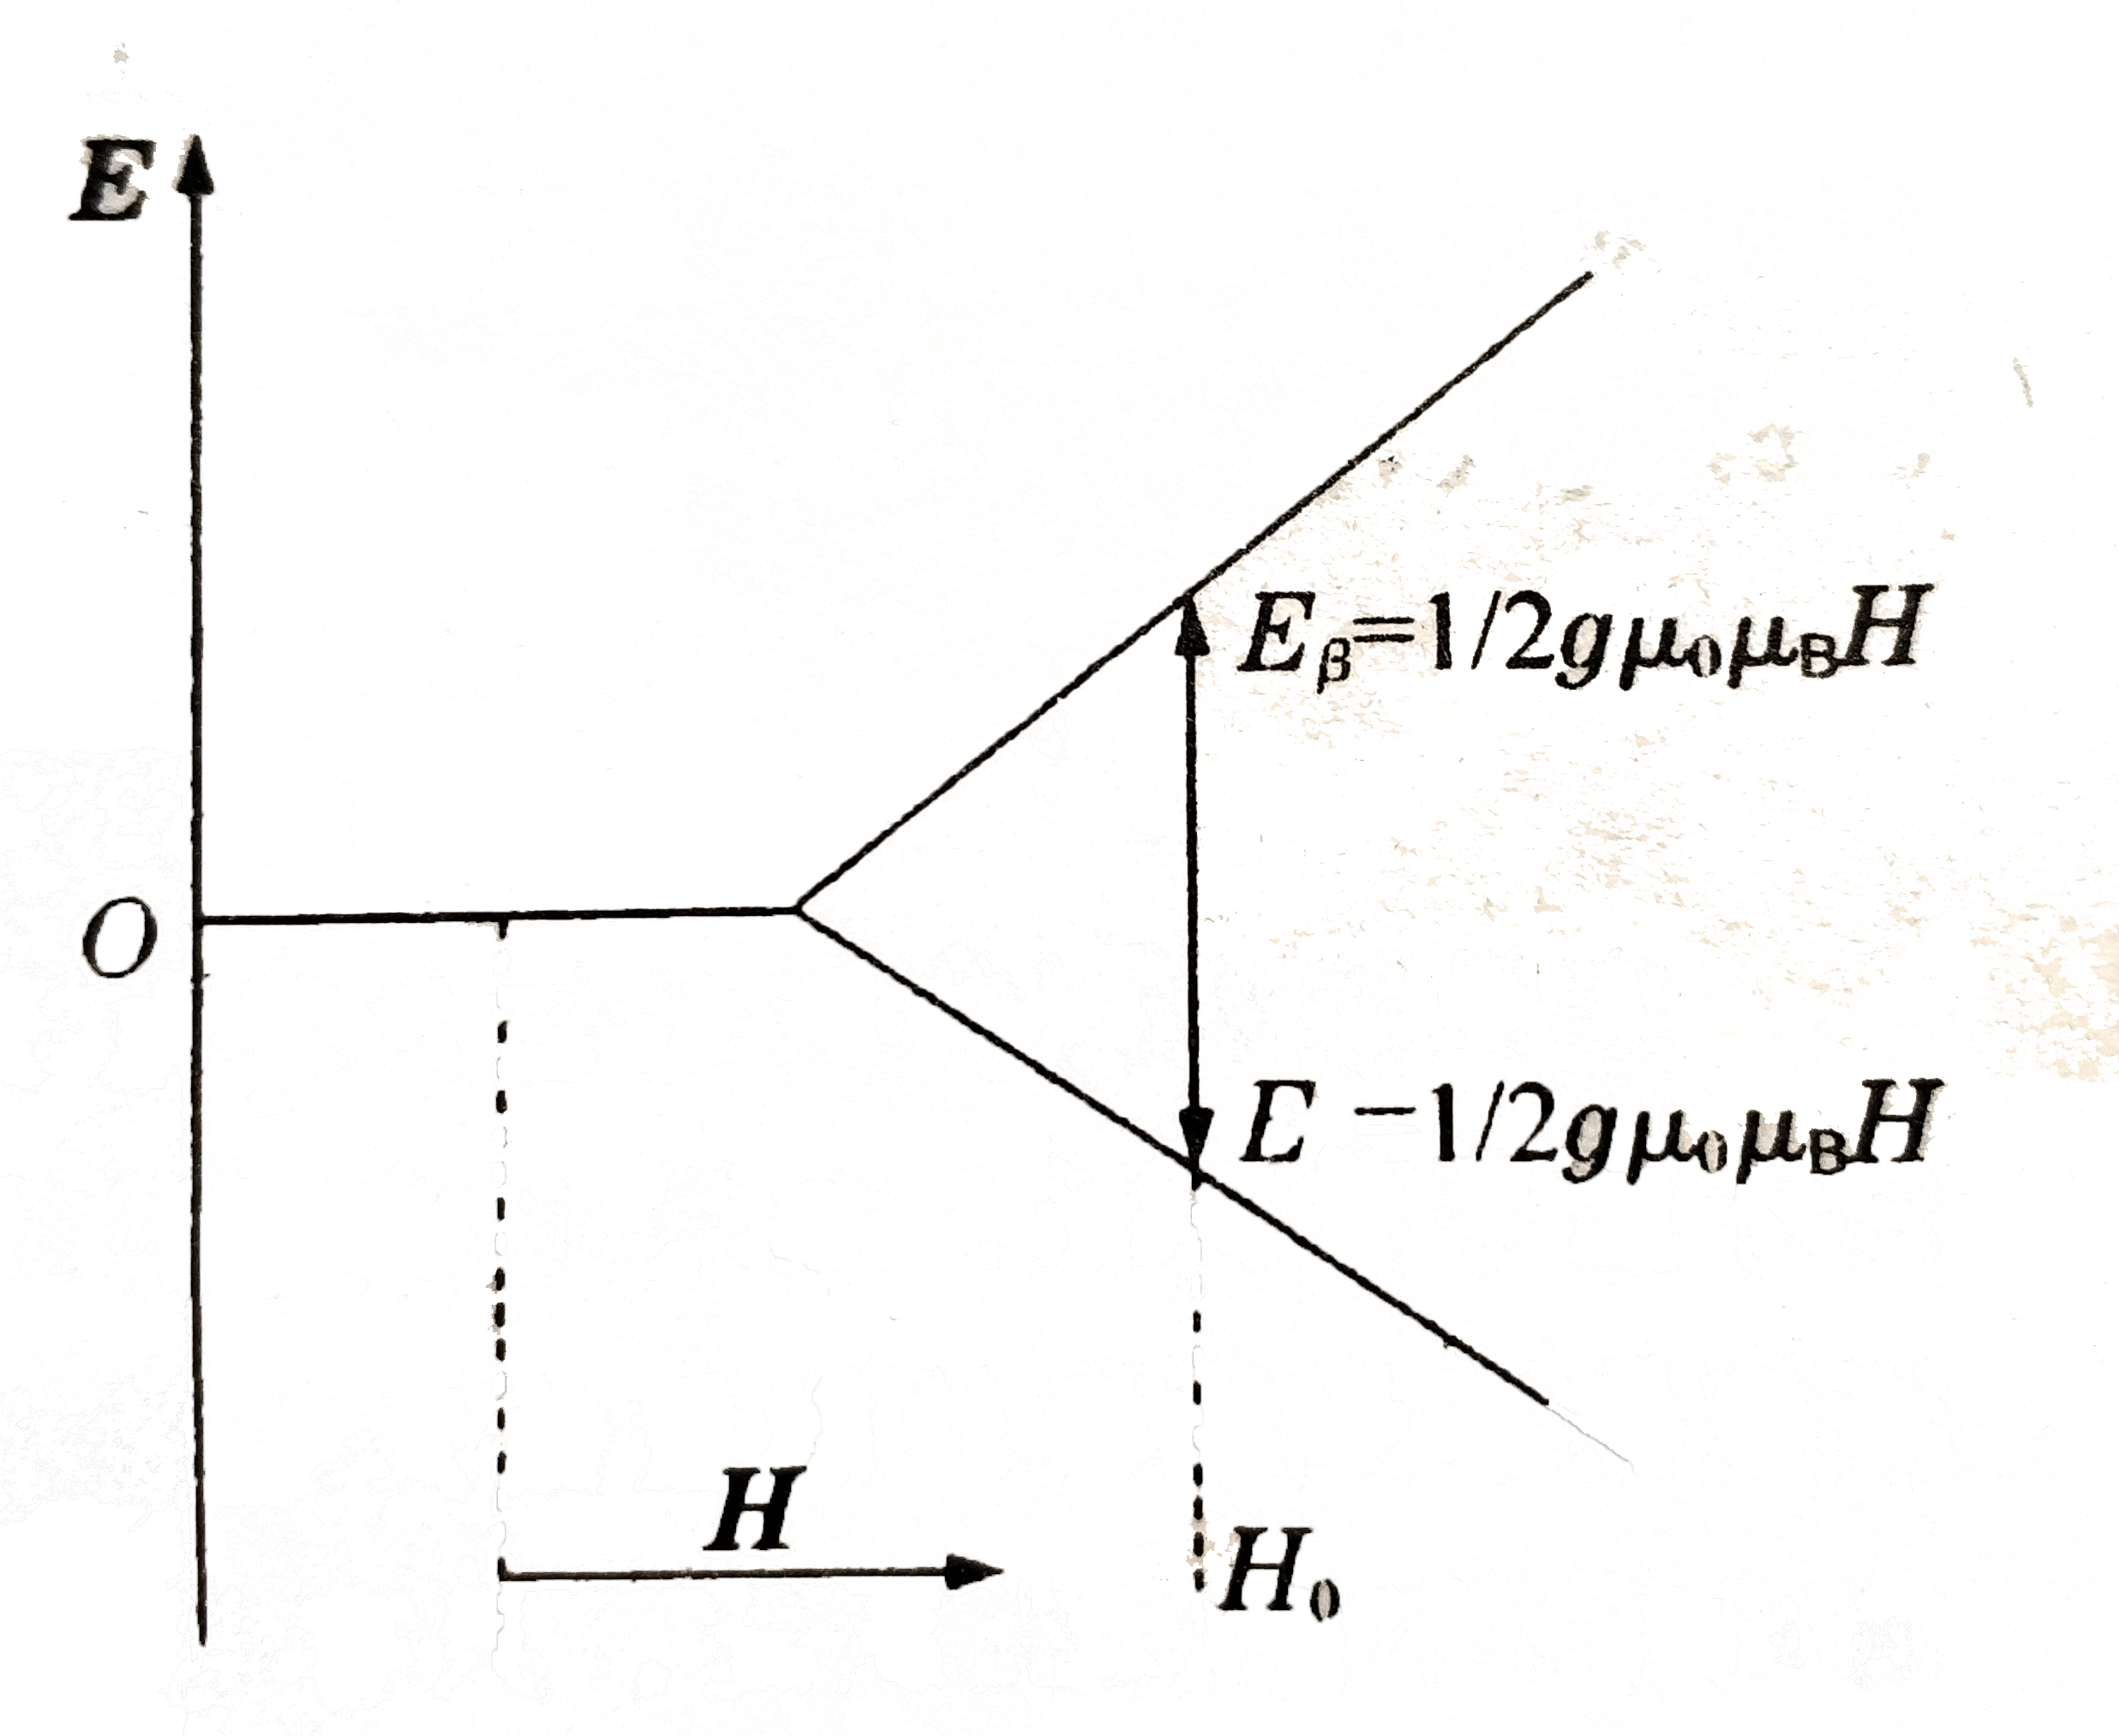
\includegraphics[width=10cm]{fig/fig1.jpg}\\
\caption{电子自旋能级与磁场强度的关系}\label{fig1}    
\end{figure}

\subsection{电子自旋磁偶极矩$\mu$在磁场$ \vb{H} $中的运动}
电子自旋磁矩绕磁场$ \vb{H} $的进动方程为
\begin{equation}
\dv{\bm\mu}{t} = -\gamma\mu\cross \vb{H}          \label{eq6}
\end{equation}
上式的解为
\begin{equation}
\mu_x = a\cos\omega_0 t  \text{, }  \mu_y = a\sin\omega_0 t  \text{, }
mu_z = Const.    \label{eq38}
\end{equation}
式中$\omega_0 = \gamma H_0$。上式表征了磁偶极矩$\mu$与磁场$H_0$保恃一定的角度绕$ z $轴做Larmor进动, 其进动的角频率为$\omega_0 = \gamma H_0$。如图(\ref{fig2})所示。
\begin{figure}[H]
\centering
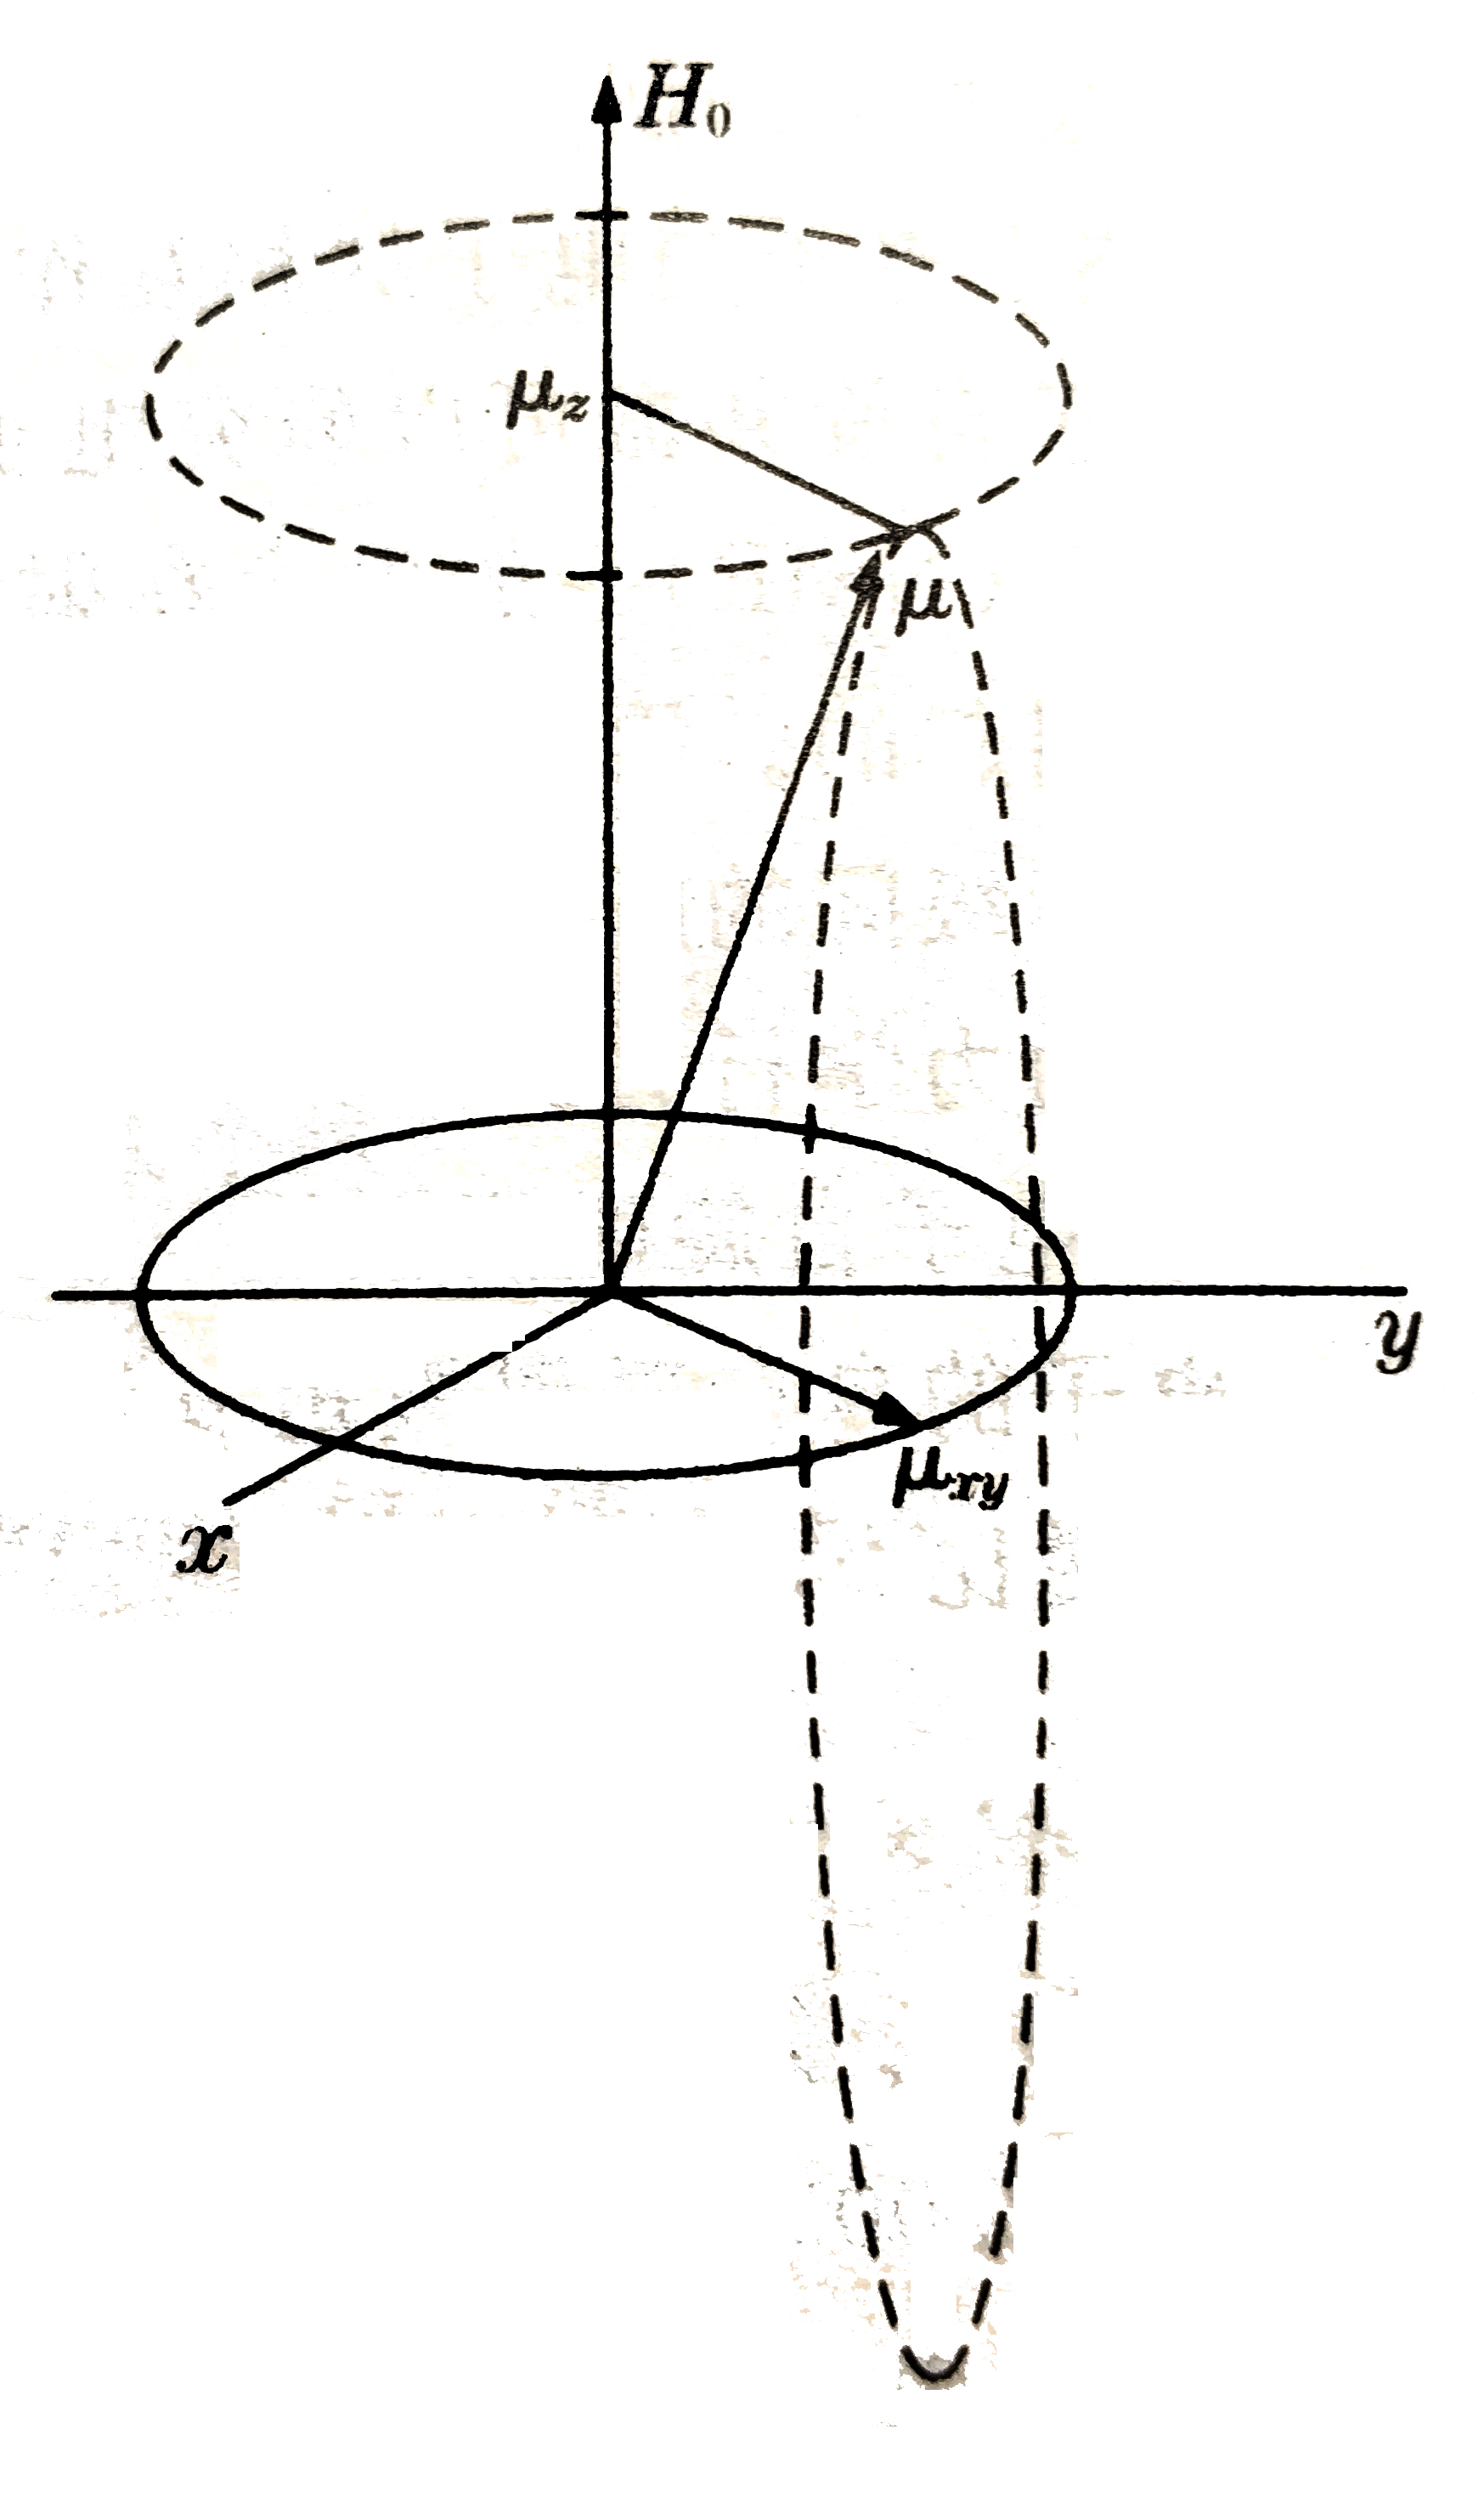
\includegraphics[width=5cm]{fig/fig2.jpg}\\
\caption{电子自旋磁矩在外场中的运动}\label{fig2}
\end{figure}
如果在垂直于恒定磁场$ \vb{H} $的平面内加进一个旋转磁场$\tilde{\vb{h}}$,若此旋转磁场的旋转方向和进动方向相冋,当$\tilde{\vb{h}}$的旋转角频率$\omega = \omega_0$时,$\bm\mu$和$\tilde{\vb{h}}$保持相对静止。于是$\bm\mu$也将受到一个力矩$ -\bm\mu\cross\tilde{\vb{h}} $的作用,绕$\tilde{\vb{h}}$做进动,结果是$\bm\mu$与$\vb{H}_0$之间的夹角增大,说明例子吸收了来自旋转磁场$\tilde{\vb{h}}$的势能,这就发生了电子顺磁共振现象,共振条件:
\begin{equation}
\omega_0 = \omega = \gamma H_0 = \dfrac{g\mu_B}{\hbar}H_0\label{eq9}
\end{equation}
由此
\begin{equation}
h\nu = g\mu_BH_0             \label{eq10}
\end{equation}
\subsection{电子自旋的量子力学描述}
自旋为S的电子
\begin{equation}
\mu_e = -g\mu_BS\label{eq11}
\end{equation}
分裂的能级间隔为:
\begin{equation}
\Delta E = g\mu_B H\label{eq12}
\end{equation}
当外加一个频率为$\nu$的交变磁场$\tilde{h}$,当满足条件:
\begin{equation}
h\nu = \Delta E = g\mu_B H\label{eq13}
\end{equation}
时,就会发生共振吸收。
g=2时,计算得共振频率为$\nu$ = 9.51GHz
\subsection{自旋弛豫}
上述的自旋共振吸收或发射的信号,只有当两个自旋能级间的粒子数存在差别时,才能检测到。由于电子在能级$E_{\alpha}(m_s = \frac{1}{2})$和$E_{\beta}(m_s = -\frac{1}{2})$间的跃迁,才能产生吸收或发射过程。这两个过程的速率与态的布居、微波能量密度以及跃迁矩阵元的平方成正比。垂直于稳定磁场$H_0$的微波振荡磁场(h$\nu$)可感应出两种形式的跃迁:从低能级($E_{\alpha}$)跃迁至高能级($E_{\beta}$)的过程是吸收能量,反之是辐射能量。由于低能级的粒子数较多,两个过程相抵的结果,吸收胜于辐射,结果是净吸收能量。这种由于微波振荡磁场所引起的跃迁称为“受激跃迁”。其结果必将导致各能级的布居数发生变化。

我们知道,当外磁场加在自旋为$\frac{1}{2}$的体系时,其能级将分裂成两个分量:
\begin{equation}
E = \pm\frac{1}{2}g\mu_B H\label{eq14}
\end{equation}
用$n_{\alpha}$和$n_{\beta}$表示上下能级的布居数。当自旋体系与晶格处于热力学平衡状态时,电子是按玻尔兹曼规律分布在两能级间,即:
\begin{equation}
\cfrac{n_{\alpha}}{N_{\beta}} = e^{\frac{-\Delta E}{k_BT}} = e^{\frac{-g\mu_B H}{k_BT}}\label{eq15}
\end{equation}
设
\begin{equation*}
N = (n_{\beta} + n_{\alpha})\text{, }n = (n_{\beta} - n_{\alpha})
\end{equation*}
设此自旋体系受微波场辐照时,其向上和向下的受激跃迁概率均为P,则$\ket{\beta}$态布居数的变化率写成
\begin{equation}
\cfrac{\text{d}n_{\beta}}{\text{d}t} = P(n_{\alpha} - n_{\beta}) = -Pn\label{eq18}
\end{equation}
即
\begin{equation}
\cfrac{\text{d}n}{\text{d}t} = -2Pn\label{eq19}
\end{equation}
解得
\begin{equation}
n = n(0)e^{-2Pt}\label{eq20}
\end{equation}
因此,从辐射场吸收能量的速率为:
\begin{equation}
\cfrac{\text{d}E}{\text{d}t} = n_{\beta}P(E_{\alpha} - E_{\beta}) + n_{\alpha}(E_{\beta} - E_{\alpha}) = nP\Delta E\label{eq21}
\end{equation}
式(\ref{eq20})表明,虽然起始的布居差值为n(0),但加上微波共振场的结果,将使这差值按指数规律衰减,乃至上下能级的布居数相等,即所谓饱和。式(\ref{eq21})表明,只有n为有限数值时,才能从辐射场吸收能量。换言之,当两能级的不成对电子的布居数变成相等后,如果没有其它的相互作用,此后就不能观察到微波能量的净吸收,即不呈现ESR信号。

实际上,我们通常所观察到的ESR信号并非瞬态的,而是稳定的。这说明自旋体系微波场辐射时,不仅发生“受激跃迁”,同时还有其它的相互作用存在,使其从不平衡状态恢复至平衡状态,这样才可能保持稳定的ESR信号。这种恢复平衡的过程称为弛豫过程。由于回复平衡通常是以指数过程,因此,用弛豫时间来表征恢复平衡的速率。弛豫现象之所以引起重视,是因为谱线形状与弛豫机理是分不开的。从分析线型可以测定许多动力学过程的速率,若用其他方法该速率难以获得。

\section{实验内容}
\subsection{观察电子自旋共振吸收现象}
测量DPPH样品,用示波器观测共振吸收峰。调节电源励磁电流,改变磁场B,使其出现共振信号。分别改变B和大幅度调制场$\tilde{B}$的大小,观察信号的变化。调节得到等间隔的共振吸收峰。

\section{注意事项}
\begin{enumerate}
\item 磁极间隙的大小确定后,不要再调整,以免损坏谐振腔。
\item 取放样品时要小心谨慎,以免损坏。
\item 特斯拉计探头避免挤压,不使用时带上保护套。
\item 励磁电流要缓慢调节,关闭励磁电源前需要将电流调至零。
\end{enumerate}

\section{实验数据}
特斯拉计测得的磁感应强度为342mT。外加磁场的频率为9.37GHz。代入式(\ref{eq13})即可求出g因子:
\begin{equation}
g_1 = \cfrac{h\nu}{\mu_B H} = \cfrac{6.626\times 10^{-34}\times 9.37\times 10^{9}}{9.274\times 10^{-24}\times 0.34102} \approx 1.9632
\end{equation}
\begin{equation}
g_2 = \cfrac{h\nu}{\mu_B H} = \cfrac{6.626\times 10^{-34}\times 9.37\times 10^{9}}{9.274\times 10^{-24}\times 0.342} \approx 1.9575
\end{equation}
查阅资料可得,g因子的理论值为$g_{th}=2+\frac{1}{137\pi} \approx 2.00232343$。可算得误差分别为:
\begin{equation}
\text{Error}(g_1) = \cfrac{1.9632 - g_{th}}{g_{th}}\times 100\% \approx -1.954\%
\end{equation}
\begin{equation}
\text{Error}(g_2) = \cfrac{1.9575 - g_{th}}{g_{th}}\times 100\% \approx -2.239\%
\end{equation}
\begin{figure}[!h]
\centering
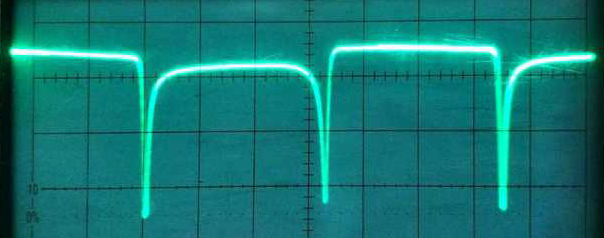
\includegraphics[width=8cm]{fig/datafig.jpg}\\
\caption{示波器上的等间隔共振峰}\label{datafig1}
\end{figure}

\begin{figure}[!h]
\centering
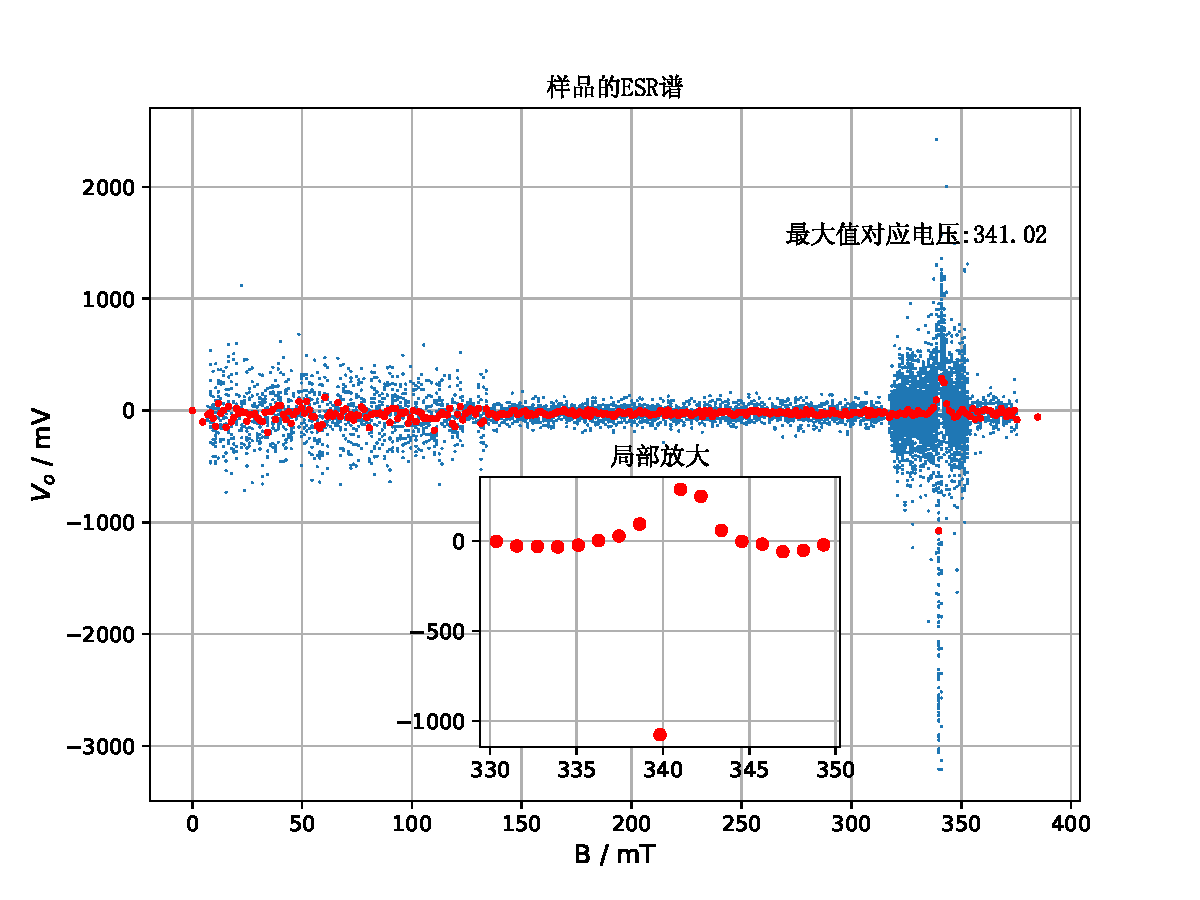
\includegraphics[width=12cm]{fig/data.pdf}\\
\caption{样品的ESR谱}\label{dataESR}    
\end{figure}

\section{思考题}
\subsection{测g值时,为什么要使共振信等间距?怎样使信号等间距?}
\subsection{$B_0$,$\tilde{B}$如何产生?作用是什么?}
\subsection{不加扫描电压能否观察到共振信号?}
\subsection{如果电脑显示的锁定放大器输出波形反相了,会是哪些原因?}
\subsection{能否用固定$B_0$,改变$\nu$的方法来测量g及B?试推导出计算公式。}

\nocite{jiaocai}
\bibliography{ref}
\end{document}